\documentclass[../AP_Physics_C/mech]{subfiles}

\begin{document}
		\section{Algebra}
			The \textbf{summation} of all terms in a data set can be denoted with just the index beneath the summation, though this need not be included for finite data sets (with the same indices).
			\[\sum_i x_i = \sum x_i\]
			\subsection{Matrices}
				A matrix is arranged as a two-dimensional rectangular array or numbers, comprised of rows ($R$) and columns ($C$). \\
				 A matrix with $m$ rows and $n$ columns can be described as being $m \times n$ ($m$ by $n$). This is its dimension. If $m$ and $n$ are equal, the matrix is a \textbf{square matrix}. \\
				 The $\th{i}$ row or column can be denoted $R_i$ or $C_i$ respectively. \\
				 Each cell of a matrix is an element. To denote the element in row $i$ and column $j$ of a matrix $A$, $A_{i,j}$ can be used.
				\[
					A = 
						\kbordermatrix{
							& C_1 & C_2 & \cdots & C_n \\
							R_1 & A_{1, 1} & A_{1, 2} & A_{1, \ldots} & A_{1, n} \\
							R_2 & A_{2, 1} & A_{2, 2} & A_{2, \ldots} & A_{2, n} \\
							\vdots & A_{\ldots, 1} & A_{\ldots, 2} & \ddots & A_{\ldots, n} \\
							R_m & A_{m, 1} & A_{m, 2} & A_{m, \ldots} & A_{m, n}
						}
 				\]
 				The \textbf{determinant} of a $2 \times 2$ matrix is the difference between the products of the diagonal terms.
 					\[\begin{vmatrix}a & b \\ c & d\end{vmatrix} = ad - bc\]
 				The determinant of a $3 \times 3$ matrix is quite similar that of a $2 \times 2$ one, using an anchor point and multiplying that by the determinant of the matrix constructed from the remaining 4 terms.
 				\[
 					\begin{vmatrix} a & b & c \\ d & e & f \\ g & h & i \end{vmatrix} = a\begin{vmatrix} e & f \\ h & i \end{vmatrix} + b\begin{vmatrix} d & f \\ g & i \end{vmatrix} + c\begin{vmatrix} d & e \\ g & i \end{vmatrix}
 				\]
 				This trend continues for \emph{square} matrices of higher dimension.
 				\subsubsection{Row Operations}
 					A \textbf{row operation} manipulates the rows of a matrix. \\
 					The \textbf{interchange} of the $\th{i}$ and $\th{j}$ rows is denoted $R_i \leftrightarrow J$. This operation simply swaps the rows.
 					\[
 						\kbordermatrix{
 							& C_1 & C_2 \\
 							R_1 & a & b \\
 							R_2 & c & d
 						} \xrightarrow{R_1 \leftrightarrow R_2}
 						\kbordermatrix{
 							& C_1 & C_2 \\
 							R_1 & c & d \\
 							R_2 & a & b
 						}
 					\]
 					\callout{8.69}{Interchange alone results in an equivalent matrix.}
 					The $\th{i}$ row can be multiplied by a scalar $k$, resulting in each of that row's elements being multiplied by $k$. This is denoted $kR_i$.
 					\[
 						\kbordermatrix{
 							& C_1 & C_2 \\
 							R_1 & a & b \\
 							R_2 & c & d
 						} \xrightarrow{kR_1}
 						\kbordermatrix{
 							& C_1 & C_2 \\
 							R_1 & ka & kb \\
 							R_2 & c & d
 						}
 					\]
 					The $\th{i}$ and $\th{j}$ rows can be added to replace either, elements in the same column being summed. Replacing $R_i$ in this way is denoted $R_i + R_j \to R_i$.
 					\[
 						\kbordermatrix{
 							& C_1 & C_2 \\
 							R_1 & a & b \\
 							R_2 & c & d
 						} \xrightarrow{R_1 + R_2 \to R_1}
 						\kbordermatrix{
 							& C_1 & C_2 \\
 							R_1 & a + c & b + d \\
 							R_2 & c & d
 						} 
 					\]
 				\subsubsection{Linear Equations}
	 				Matrices can be used to solve systems of linear equations in any number of dimensions.
					To represent a linear equation with an \textbf{augmented matrix}, the each element of a row should correspond to the coefficient of a variable with the exception of the last column's element corresponding to a constant.
	 				\[
	 					a_1x_1 + a_2x_2 + \ldots + a_nx_n = A \equiv
	 						\hspace{-2.5mm}\kbordermatrix{
	 							& x_1 & x_2 & \cdots & x_n  & & c\\
	 							& a_1 & a_2 & \cdots & a_n & \vrule & A
	 						}
	 				\]
	 				A \textbf{system of linear equations} with $m$ equations and $n$ dimensions can also be represented via an augmented matrix using row operations.
	 				\[
		 					\begin{aligned}
		 						a_{1, 1}x_1 + a_{1, 2}x_2 + \ldots + a_{1, n}nx_n &= A_1 \\
		 						a_{2, 1}x_1 + a_{2, 2}x_2 + \ldots + a_{2, n}nx_n &= A_2 \\
		 						&\hspace{6.75mm}\vdots \\
		 						a_{m, 1}x_1 + a_{m, 2}x_2 + \ldots + a_{m, n}nx_n &= A_m \\
		 					\end{aligned}
	 					\equiv
	 						\kbordermatrix{
	 							& x_1 & x_2 & \cdots & x_n & & c \\
	 							a_1 & a_{1, 1} & a_{1, 2} & a_{1, \ldots} & a_{1, n} & \vrule & A_1 \\
	 							a_2 & a_{2, 1} & a_{2, 2} & a_{2, \ldots} & a_{2, n} & \vrule & A_2 \\
	 							\vdots & a_{\ldots, 1} & a_{\ldots, 2} & \ddots & a_{\ldots, n} & \vrule & \vdots \\
	 							a_m & a_{m, 1} & a_{m, 2} & a_{m, \ldots} & a_{m, n} & \vrule & A_m
	 						}
	 				\]
 				\subsubsection{Matrix Operations}
 					
			\subsection{Vectors}
				A \textbf{scalar} is a quantity with only magnitude. \\
				A \textbf{vector} is a quantity with both magnitude and direction. A vector is denoted by an arrow ($\to$) above the variable. It can be represented by a 1-row matrix. \\
				A vector can be divided into \textbf{components}, denoting its values in a given direction.\footnote{The interpretation of vector components denoting directions should only be used by default. This may change, especially outside of physics.} A specific component can be denoted using the vector variable (without the arrow) with the subscript of the direction ($x$, $y$, or $z$).\footnote{When the components of a vector do not denote direction, its components can be denoted by their indices in the subscript.} \\
				A vector can be denoted in \textbf{component form} by angled brackets, commas separating each component. The components are always ordered $x$, $y$, and $z$. \\
				\[\vec{v} = \langle v_x, v_y, v_z \rangle\]
				\textbf{Unit vectors} are vectors of magnitude 1 that have only a single component. The unit vectors in the $x$, $y$, and $z$ directions are $\iv$, $\jv$, and $\kv$ respectively.
				\begin{align*}
					\iv &= \langle 1, 0, 0 \rangle & 
						\jv &= \langle 0, 1, 0 \rangle & 
						\kv &= \langle 0, 0, 1 \rangle
				\end{align*}
				\textbf{Unit vector notation} breaks a vector into the sum of multiples of $\iv$, $\jv$, and $\kv$.
				\[\vec{v} = v_x\iv + v_y\jv + v_z\kv\]
				The sum of two vectors is the sum of their corresponding components and is itself a vector.
				\[\vec{u} + \vec{v} = (u_x + v_x)\iv + (u_y + v_y)\jv + (u_z + v_z)\kv\]
				The \textbf{magnitude} of a vector, denoted by enclosing the vector within four vertical lines, is the square root of the sum of the squares of its components. It is a \emph{scalar} quantity.
				\[||\vec{v}|| = \sqrt{\sum_{i = 1}^n v_i^2} = \sqrt{v_x^2 + v_y^2 + v_z^2}\]
				To add two vectors graphically, the tip of one can be attached to the tail of the other, and the \textbf{resultant vector} can be drawn along the hypotenuse of the formed triangle.
				\begin{center}
					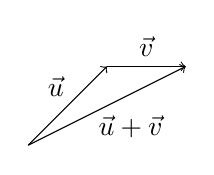
\begin{tikzpicture}
						\draw[->] (0, 0) -- node[above]{\hspace{-3mm}$\vec{u}$} ++ (1, 1);
						\draw[->] (1, 1) -- node[above]{$\vec{v}$} ++ (1, 0);
						\draw[->] (0, 0) -- node[below]{\hspace{6mm}$\vec{u} + \vec{v}$} ++ (2, 1);
					\end{tikzpicture}
				\end{center}
				The \textbf{dot product} of two vectors, denoted by a dot, is the sum of the products of their corresponding components. This is a \emph{scalar} quantity.
				\[\vec{u} \cdot \vec{v} = \sum_{i = 1}^n u_iv_i= u_xv_x + u_yv_y + u_zv_z\]
				The \textbf{cross product} of two vectors, denoted by a cross, is the 
		\section{Calculus}
\end{document}